% Bisher nur Notizen
% also nicht viel verwertbares

\chapter{Beispiele/Anwendung}
\section{Einfache Beispiele}
%\subsection{erstes}
\[
  P_a=t^2\partial_t^2+t\partial_t+(t^2-n^2)=\sum_{k=0}^2\sum_{l=0}^2
  \alpha_{kl}t^l\partial_t^k
\]

Mit: $\alpha_{2,2}=1$, $\alpha_{1,1}=1$, $\alpha_{0,2}=t^2$ und
$\alpha_{0,0}=n^2$

$
P_a=t^2\partial_t^2+t\partial_t+(t^2-n^2) \Rightarrow 
\begin{cases}
  k=2,l=2 & \Rightarrow u\leq k=2, v\geq l-k=0\\
  k=1,l=1 & \Rightarrow u\leq 1, v\geq 0\\
  k=0,l=0 & \Rightarrow u\leq 0, v\geq 0\\
  k=0,l=2 & \Rightarrow u\leq 0, v\geq 2\\
\end{cases}
$

\begin{center}
  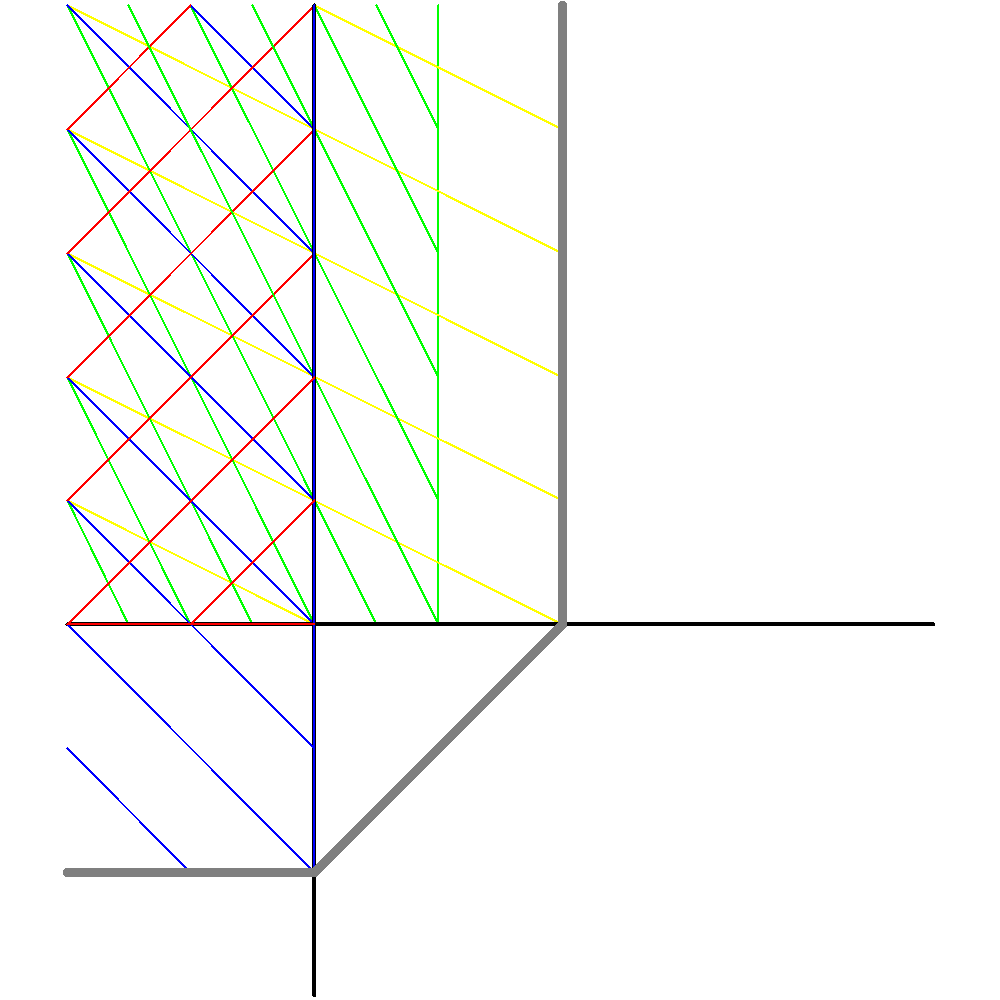
\includegraphics[width=6cm]{beispiele/img/a.png}
\end{center}
also $\slopes(P_a)=\{0\}$ also ist $P_a$ regulär singulär

% vim: set ft=tex :
 % nur ein slope: 1
%\subsection{zweites}
\[
  P_b=t\partial_t^2+2\partial_t-1
\]

$
P_b=t\partial_t^2+2\partial_t-1 \Rightarrow 
\begin{cases}
  k=2,l=1 & \Rightarrow u\leq l=2, v\geq l-k=-1\\
  k=1,l=0 & \Rightarrow u\leq 1, v\geq -1\\
  k=0,l=0 & \Rightarrow u\leq 0, v\geq 0\\
\end{cases}
$

\begin{center}
  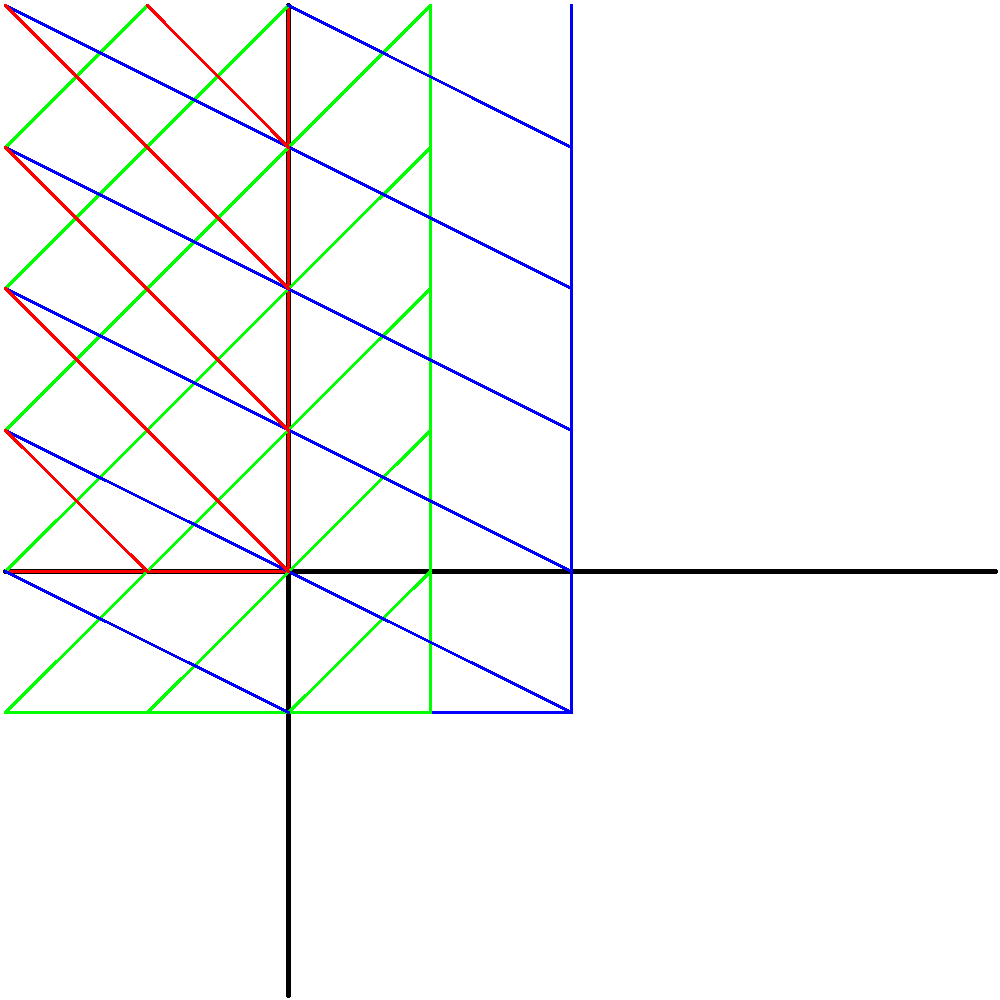
\includegraphics[width=6cm]{beispiele/img/b.png}
\end{center}
also $\slopes(P_b)=\{0\}$ also ist $P_b$ regulär singulär

% vim: set ft=tex :
 % regulär singulär
%\subsection{drittes}

\begin{comment}
  zula Barbara Seite 46
\end{comment}


\[
  P_c=t^2\partial_t+1
\]
$
P_c=t^2\partial_t+1
\Rightarrow
\begin{cases}
  k=1, l=2 & \Rightarrow u \leq 1, v \geq 1\\
  k=0, l=1 & \Rightarrow u \leq 0  v \geq 0\\
\end{cases}
$
\begin{center}
  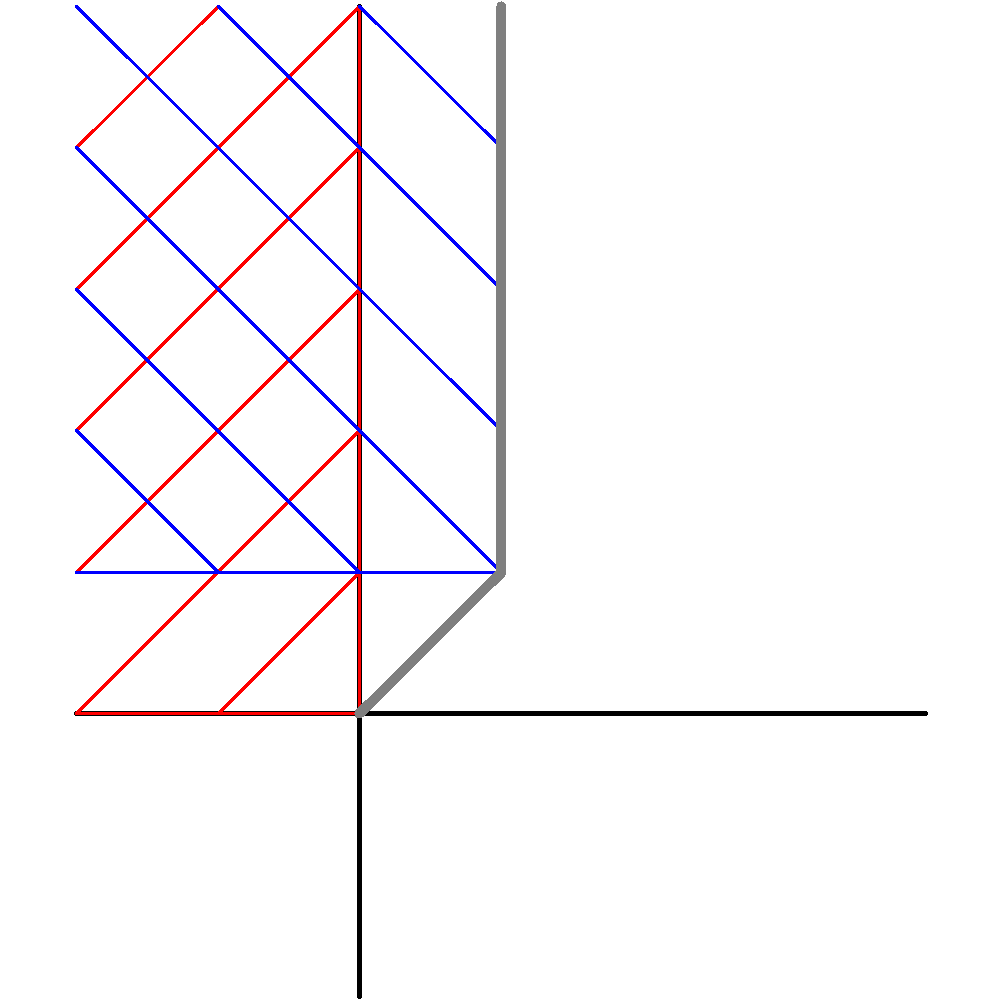
\includegraphics[width=6cm]{beispiele/img/c.png}
\end{center}

also $\slopes(P_c)=\{1\}$.

% vim:set ft=tex :
 % nur ein slope: 1
%\subsection{viertes}

\begin{comment}
  zula Barbara Seite 46
\end{comment}

\begin{comment}
  Original aus der Zula:
  \[
    P_d=-3t^{14}\partial_t^6+t^{11}(t+3)\partial_t^5 + 2t^8\partial_t^4
    -t^6(t^3+1)\partial_t^3 + t^4\partial_t
  \]

  $ P_d \Rightarrow
  \begin{cases}
    k=6,l=14 & \Rightarrow u\leq k=6, v\geq l-k=8\\
    k=5,l=12 & \Rightarrow u\leq 5, v\geq 7\\
    k=5,l=11 & \Rightarrow u\leq 5, v\geq 6\\
    k=4,l=8 & \Rightarrow u\leq 4, v\geq 4\\
    k=3,l=9 & \Rightarrow u\leq 3, v\geq 6\\
    k=3,l=6 & \Rightarrow u\leq 3, v\geq 3\\
    k=1,l=4 & \Rightarrow u\leq 1, v\geq 3\\
  \end{cases} $

  also ist Abbildung 5.8 auf seite 53 der zula falsch?
\end{comment}

\[
  P_d=-3t^{14}\partial_t^6+t^{11}(t+3)\partial_t^5 + 2t^8\partial_t^4
  -t^6(t^3+1)\partial_t^3 + t^3\partial_t
\]

$ P_d \Rightarrow
\begin{cases}
  k=6,l=14 & \Rightarrow u\leq k=6, v\geq l-k=8\\
  k=5,l=12 & \Rightarrow u\leq 5, v\geq 7\\
  k=5,l=11 & \Rightarrow u\leq 5, v\geq 6\\
  k=4,l=8 & \Rightarrow u\leq 4, v\geq 4\\
  k=3,l=9 & \Rightarrow u\leq 3, v\geq 6\\
  k=3,l=6 & \Rightarrow u\leq 3, v\geq 3\\
  k=1,l=3 & \Rightarrow u\leq 1, v\geq 2\\
\end{cases} $

\begin{center}
  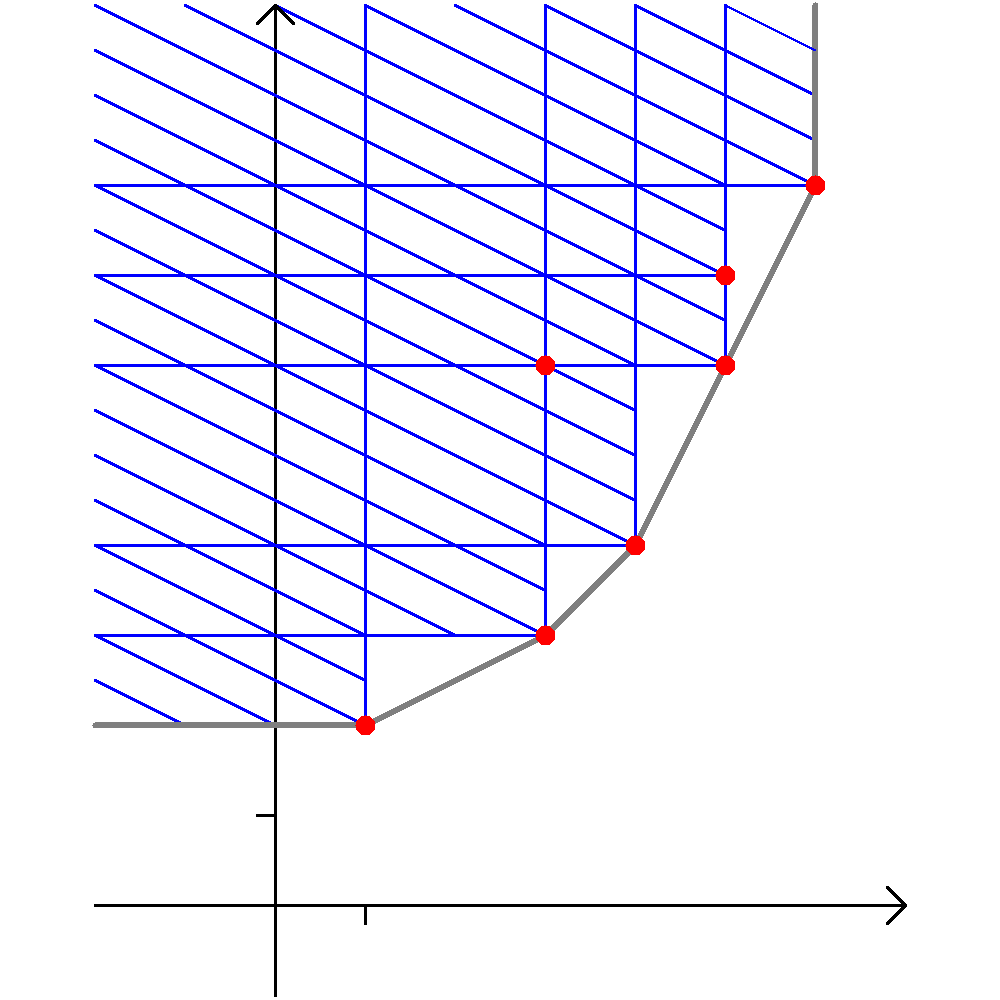
\includegraphics[width=6cm]{beispiele/img/d.png}
\end{center}
also $\slopes(P_b)=\{0,\frac{1}{2},1,2\}$ also ist $P_d$ irregulär singulär.\\
Offenbar ist der Hauptnenner der Steigugnen gleich $2$.\\
Betrachte also $\rho:t\mapsto u^2$\\
und erhalte: ???

% vim: set ft=tex :
 % zu kompliziert
%\subsection{bsp e}

\[
  P_e=t^4(t+1)\partial_t^4 + t\partial_t^2+\frac{1}{t}\partial_t+1
\]

\begin{center}
  \includegraphics[width=6cm]{beispiele/img/e.png}
\end{center}

also $\slopes(P_e)=\{0,\frac{2}{3}\}$

Dies gilt Analog für das einfachere:
\[
  \bar P_e=t^4\partial_t^4 +\frac{1}{t}\partial_t
\]

\begin{center}
  \includegraphics[width=6cm]{beispiele/img/bar_e.png}
\end{center}

% vim: set ft=tex :
 % verbesserte version: e_new
%Neuer versuch, ein geeignetes Beispiel zu finden

Hier soll ein einfaches Beispiel hergeleitet werden, an dem die Zerlegung nach
dem Levelt-Turittin-Theorem einmal explizit ausformuliert werden soll.

Beginne mit

\begin{minipage}[hbt]{0,49\textwidth}
  \[ t^4(t+1)\partial_t^4 + t\partial_t^2+\frac{1}{t}\partial_t+1 \]
\end{minipage}
\begin{minipage}[hbt]{0,49\textwidth}
  \begin{center}
    \includegraphics[width=3cm]{img/e.png}
  \end{center}
\end{minipage}

(von ZulaBarbara Seite 47)
und ignoriere zuerst die Terme, die zum Newton Polygon keinen Beitrag leisten

\begin{minipage}[hbt]{0,49\textwidth}
  \[ t^4\partial_t^4 +\frac{1}{t}\partial_t \]
\end{minipage}
\begin{minipage}[hbt]{0,49\textwidth}
  \begin{center}
    \includegraphics[width=3cm]{img/bar_e.png}
  \end{center}
\end{minipage}

multipliziere dieses mit $t$ und ändere aber dadurch den assoziierten
Meromorphen Zusammenhang nicht \cite[Chapter 5.1]{sabbah_cimpa90}

\begin{minipage}[hbt]{0,49\textwidth}
  \[ P:=t^5\partial_t^4 +\partial_t \]
\end{minipage}
\begin{minipage}[hbt]{0,49\textwidth}
  \begin{center} 
    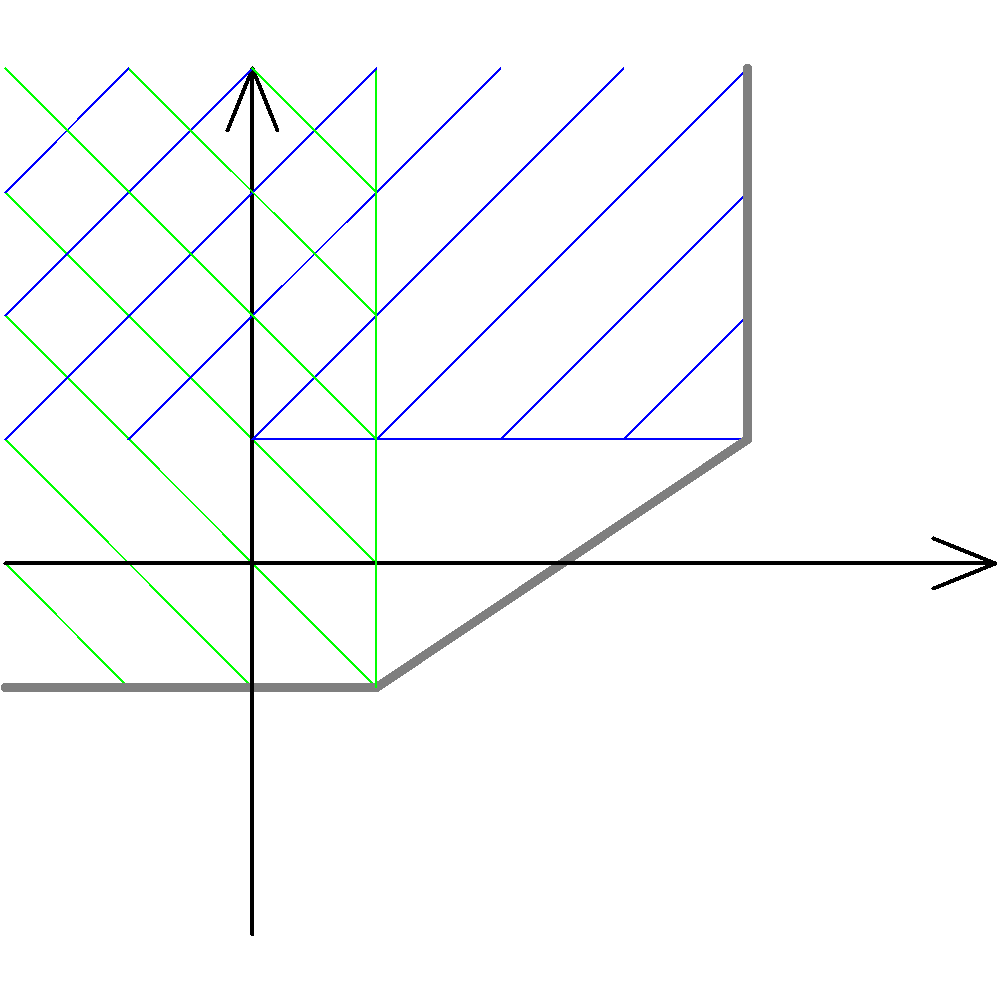
\includegraphics[width=3cm]{img/bar_e_times_x.png} 
  \end{center}
\end{minipage}

und es gilt $\slopes(P)=\{0,\frac{2}{3}\}$. Eliminiere als nächstes nun die
Brüche in den Slopes mittels einem geeignetem Pullback. Da hier der Hauptnenner
$3$ ist bietet sich $\rho:t\mapsto u^3$ für den Pullback an.
\begin{comment}
  Dieser Pullback Multipliziert (indirekt) die Slopes mit $3$,
  \textbf{Quelle?}\\ aber wie wendet man ihn (explizit) an?
\end{comment}

\[ \rho^+P=??? \]
welches die Slopes $\slopes(\rho^+P)=\{0,2\}\subset\Z$ hat. Schreibe nun dieses
$\rho^+P=Q\cdot R$ mit $P,Q\in\Cfu$ wobei gilt $\slopes(Q)=\{0\}$ und
$\slopes(R)=\{2\}$.

Also gilt:
\[
  \hat\cD/(\hat\cD\cdot\rho^+P)\cong
  \hat\cD/(\hat\cD\cdot Q) \oplus  \hat\cD/(\hat\cD\cdot R)
\]

% vim: set ft=tex :

\section{Meromorpher Zusammenhang der formal, aber nicht Konvergent, zuerfällt}
\begin{comment}
  Quellen??
  \[
    \sum n!x^n
  \]
\end{comment}

% eine Übungsaufgabe aus sabbah_cimpba90 Seite 33
% 5.3.6
% 
% zwefällt formal aber NICHT konvergent

\subsection{beispiel von sabbah}

Sei $P=t(t\partial_t)^2+t\partial_t+\frac{1}{2}$

\begin{comment}
  \begin{enumerate}
      \item zeige $\cD/\cD\cdot P$ ist ein Meromorpher Zusammenhang.
      \item Zeichne das Newton Polygon von $P$ und finde eine formale
        Aufteilung von $\cM_{\hat{K}}$.
      \item Zeige $\cM$ kann nicht in eine direkte Summe von zwei $\cD$ modulen
        zerlegt werden, dazu:
        \begin{enumerate}
          \item Zeige das die Produktzerlegung
            \[ P=(t(t\partial_t)+v(t))\cdot(t\partial_t+u(t)) \,, \]
            mit $u,v\in\Cfu$, existiert.
          \item Berechne durch Induktion die Koeffizienten von $u$.
          \item Zeige dass $u \notin \C((u))$.
        \end{enumerate}
  \end{enumerate}
\end{comment}

\subsubsection{Schritt 1} Zeige das $\cD/\cD\cdot P$ einen Meromorphen
Zusammenhag Definiert.
\subsubsection{Schritt 2}
\begin{minipage}[hbt]{0,39\textwidth}
  \begin{align*}
   P &= t(t\partial_t)^2                + t\partial_t           + \frac{1}{2}\\
     &= tt(\partial_tt)\partial_t       + t\partial_t           + \frac{1}{2}\\
     &= t^2(t\partial_t + 1)\partial_t  + t\partial_t           + \frac{1}{2}\\
     &= t^3\partial_t^2                 + (t^2 + t)\partial_t   + \frac{1}{2}\\
  \end{align*}
\end{minipage}
\begin{minipage}[hbt]{0,59\textwidth}
  \begin{center}
    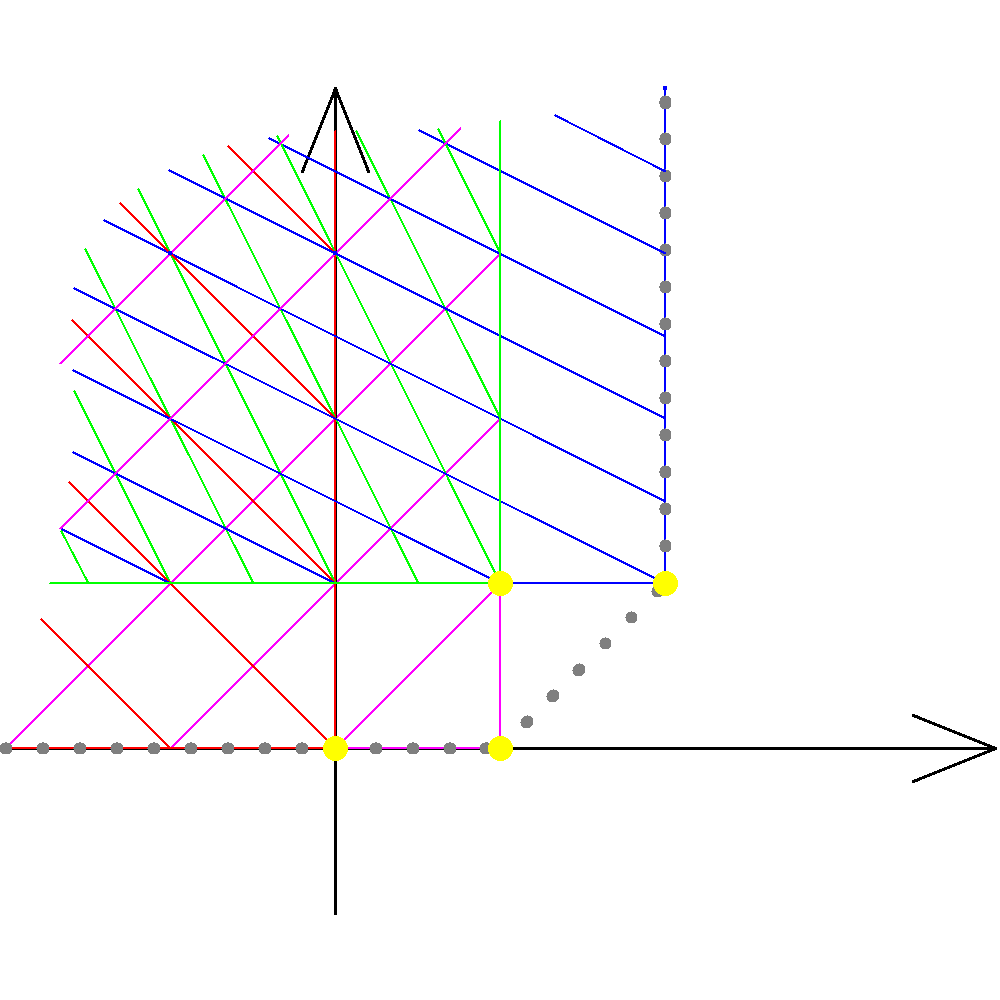
\includegraphics[width=6cm]{img/formal_a-2.png}
  \end{center}
\end{minipage}
Also mit $\slopes{P}=\{0,1\}$

\subsubsection{Schritt 3 a)}
\subsubsection{Schritt 3 b)}
\subsubsection{Schritt 3 c)}

% vim: set ft=tex :


\begin{comment}
  Weiteres Beispiel:
  \[
    Sabbah\_Fourier-local.pdf \rightarrow 5.b.
  \]
\end{comment}

% vim: set ft=tex :
